\chapter{Future Plans}
\section{Communication}
While it is possible to transfer information easily between robots since a simulator is used one keypoint was to try implement it as close to a realistic scenario as possible, meaning that the communication range for the robots is limited. In an realistic scenario every robot would have to send the acquired map back to the static start point/lead robot so that an overall map of the environment can be created. \\
Since the communication range for such small robots is limited and can be even further obstructed through obstacles like walls it is important to designated some robots as communication nodes. Such comm nodes would than remain stationary and link the "scout" robots, which do the exploration, back to do the lead robot. \\
Obviously the most effective way to do this is by implementing different behaviour patterns for scouts or comm robots, and implement a decision model which allows the robot to change between either pattern as the needs of the swarm change. E.g. in the start of the exploration no comm robots will be needed as the robots would most likely be inside the comm range of the lead robot, though this may change if the swarm is big and spread out enough. \\[3ex]

To surpass the problems of obstacles obstructing the communication the comm robots would need to position them self on logical places i.e. in order to scan a room it would be important that a comm robot places it self inside, or close to, the doorway so that others can explore the room and still communicated back to the rest of the swarm. The robot would need to stay inside the doorway as signals can not always travel through walls and the energy reserves of mobile robots are limited so they most likely can not send high power signals. \\
It has not been decided how this would be implemented since as of now it is not sure if the E-puck models implemented inside the simulator are able to send signals to other robots. While it is possible  to transfer signals through the E-puck's laser sensors it is not know if this would actually be a better implementation than using radio transmitters and receivers.\\[3ex]

The theory of what could be  implemented uses a defined maximum communication range for the robots and a grouping strategy which specifies that each scout robot need to stay in contact which at least 1 comm robot while the comm robots always need at least 1 other comm robot inside their communication range. If implemented correctly the comm robots would on this way create a communication link back to the lead robot/starting location which the scout robots can use to transfer all new information back.\\

\begin{figure}[h]
\centering
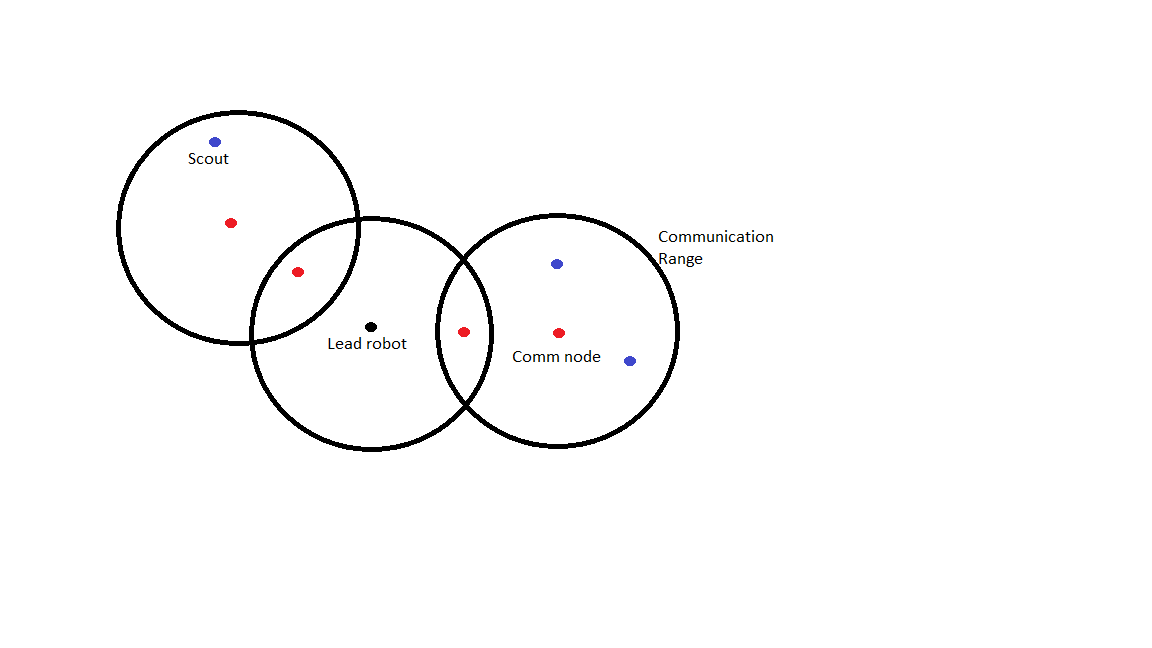
\includegraphics[width = 0.8\textwidth]{../../figures/comm_example.png} 
\caption{An example of the communication link}
\label{Figure 1}
\end{figure}

Figure 1 shows one possible example of the communication link, where the lead robot/ or in some cases a stationary uplink point is in the center and the communication robots(in red) placed in such positions that their comm range overlaps the comm range of other robots and the lead robot. \\
This configuration allows the scouts(in blue) to move and explore anything inside the communication range of the different comm robots. When the robots at the right side of the figure would now try to move outside the comm range one of them would have to change their behaviour pattern to "communication mode" at the outer range of the other comm nodes range while the last remaining scout continuous exploring in this direction. \\
This example shows that it is important to have a swarm of a suitable size for an environment to be able to cover at much area with the robots at hand and for cases in which this is not possible to be able to move the whole swarm in one unified direction to explore unmapped locations. This is however only doable when there is a lead robot since a stationary comm/uplink point is by definition, stationary.\\